% Author - - Jon Arnt Kårstad, NTNU IMT
\documentclass{article}

% Importing document settings from our file "packages.sty"
\usepackage{packages}

% Beginning of document
\begin{document}

% Inserting title page
\import{./}{title}

% Defining front matter settings 
\frontmatter

% Inserting table of contents
\tableofcontents

% Inserting list of figures & list of tables
\listoffigures
\listoftables

% Defining main matter settings
\mainmatter

\section{Motivation}
    \import{./Sections/}{Zusammenfassung}

\section{Introduction}
    \import{./Sections/Introduction}{Introduction}

    \subsection{OOP Design Patterns}
        \import{./Sections/Introduction/OOPDesignPatterns}{OOPPatterns}

        \subsubsection{Observer}
            \import{./Sections/Introduction/OOPDesignPatterns/sub/}{Observer}

        \subsubsection{Proxy}
            \import{./Sections/Introduction/OOPDesignPatterns/sub/}{Proxy}

        \subsubsection{TemplateMethod}
            \import{./Sections/Introduction/OOPDesignPatterns/sub/}{TemplateMethod}

        \subsubsection{Builder}
            \import{./Sections/Introduction/OOPDesignPatterns/sub/}{Builder}

        \subsubsection{Facade}
            \import{./Sections/Introduction/OOPDesignPatterns/sub/}{Facade}

    \subsection{CleanArchitecture}
        \import{./Sections/Introduction/CleanArchitecture}{CleanArchitecture}

    \subsection{Software Testing}
        \import{./Sections/Introduction/SoftwareTesting}{SoftwareTesting}

        \subsubsection{Testing Pyramide}
            \import{./Sections/Introduction/SoftwareTesting/sub/}{TestingPyramide}
        
        \subsubsection{Unit Tests}
            \import{./Sections/Introduction/SoftwareTesting/sub/}{UnitTests}
        
        \subsubsection{Integration Tests}
            \import{./Sections/Introduction/SoftwareTesting/sub/}{IntegrationTests}

        \subsubsection{SystemTests}
            \import{./Sections/Introduction/SoftwareTesting/sub/}{SystemTests}

        \subsubsection{UI Tests}
            \import{./Sections/Introduction/SoftwareTesting/sub/}{uitests}

        \subsubsection{Manual Tests}
            \import{./Sections/Introduction/SoftwareTesting/sub/}{ManualTests}

    \subsection{SOLID}
        \import{./Sections/Introduction/SOLID/}{SOLID}

        \subsubsection{single-responsibility principle}
            \import{./Sections/Introduction/SOLID/sub/}{SingleResponsibilityPrinciple}
        
        \subsubsection{open–closed principle}
            \import{./Sections/Introduction/SOLID/sub/}{OpenClosedPrinciple}
        
        \subsubsection{Liskov substitution principle}
            \import{./Sections/Introduction/SOLID/sub/}{LiskovSubstitutionPrinciple}
        
        \subsubsection{interface segregation principle}
            \import{./Sections/Introduction/SOLID/sub/}{InterfaceSegregationPrinciple}
        
        \subsubsection{dependency inversion principle}
            \import{./Sections/Introduction/SOLID/sub/}{DependencyInversionPrinciple}

    \subsection{GRASP}
        \import{./Sections/Introduction/GRASP/}{GRASP}

    \subsection{OOP Principles}
        \import{./Sections/Introduction/OOPPrinciples/}{OOPPrinciples}

        \subsubsection{Abstraction}
            \import{./Sections/Introduction/OOPPrinciples/sub}{Abstraction}

        \subsubsection{Encapsulation}
            \import{./Sections/Introduction/OOPPrinciples/sub}{Encapsulation}

        \subsubsection{Inheritance}
            \import{./Sections/Introduction/OOPPrinciples/sub}{Inheritance}

        \subsubsection{Polymorphism}
            \import{./Sections/Introduction/OOPPrinciples/sub}{Polymorphism}

\newpage

\section{Software Architektur}

    \subsection{Was ist eine Software Architektur}

    Bevor man anfängt über die Software Architectur zu reden, muss man sie erstmal definieren.
    Es gibt keine einheitliche Definition einer Software Architectur. Verschiedene Authoren definieren es auch unterschiedlich.

    Robert Martin definiert es als ein Gegenstand mit bestimmten Eigenschaften zu definieren.\\
    \textit{Softwarearchitektur ist die Gestalt des Systems erstellt von derjenigen, die das entwickeln. 
    Die Form dieser Gestalt ist das Aufteilen des Systems in Komponenten, die Anordnung (Arrangement) dieser Komponenten und die Wege, 
    wie diese Komponente miteinander kommunizieren} \cite[136]{cleanArchitecture}
    
    Ralph Jonson definiert Software Architecture aus Sicht eines Projektes.\\
    \textit{Architecture besteht aus den Entscheidungen, die man sich wünscht so früh wie möglich in einem Projekt zu treffen}
    \cite{MF_WhatIsSA}

    In dem ersten Teil des Kapitels wird die Softwarearchitektur aus Sicht eines Projektes betrachtet, 
    indem es kurz beschrieben wird, welche Auswirkungen eine gute und eine schlechte Architektur auf ein Projekt haben kann.

    In dem 2. Teil des Kapitels, wird die Architecture des OCPP Backend Serves beschrieben
    \begin{itemize}
        \item in welche Teile das Programm aufgeteilt wurde
        \item Testbarkeit und Erweitbarkeit einzelner Teile des Programms
        \item wie die einzelnen Teile miteinander kommunizieren
    \end{itemize}

    \subsection{Ziele der Software Architektur}

    \textit{Das Ziel der Software Architektur ist das Mininimieren der menschlichen Ressourcen, 
    die benötigt werden um ein System zu entwickeln und zu unterstützen.}\cite[5]{cleanArchitecture}

    Diese Aussage lässt sich sehr einfach überprüfen, indem man feststellt, 
    ob jede neue Anforderungen an der Software mehr Ressourcen verbraucht als die vorherigen.

    \textit{Das Ziel der Softwarearchitektur ist so viel Entscheidungen wie möglich so spät wie möglich zu treffen}
    \cite[136]{cleanArchitecture}

    Beispiele für solche Entscheidungen wären:
    \begin{itemize}
        \item Datenbanksystem
        \item Transferprotokoll zu der Benutzeroberfläche (z.B. HTTP oder WS) falls vorhanden
        \item Wie und wo die Loggingdaten gespeichert werden (in einer Datei, Datenbank oder externe Server)
    \end{itemize}

    Auch die Tätigkeiten, die nicht mit Programmieren direkt zu tun haben, werden von den Entscheidungen in der Softwarearchitektur betroffen
    \begin{itemize}
        \item Deployment (Aufsetzung) der Software.
        \item Maintenance (Unterstützung) der Software.
    \end{itemize}

    Deployment der Software beinhaltet die Kosten die durch das Aufsetzen der neuen Version der Software entstehen.\\
    Maintenance der Software beinhaltet die Kosten, die nach dem Beenden der Entwicklung bei kleineren Erweiterungen und Änderungen des Systems entstehen.


    \subsection{Technische Schulden}
    Bei den Änderungen oder Erweiterungen eines Systems oft entsteht ein Overhead, das durch die "Unsaubarkeit" des bestehenden Programms verusacht wird.

    Dieses Overhead wird als technische Schulden (en. : Technical Debts) bezeichnet.

    Die technischen Schulden entstehen dadurch, dass bei der Entwicklung eines Teiles des Systems wurde 
    von den Entwicklungsteam weniger Zeit investiert um die nicht Gewinnbringende Sachen zu implementieren.
    Beispiele für solche Tätigkeiten wären:
    \begin{itemize}
        \item Unittests
        \item Dokumentieren 
        \item Code Review
    \end{itemize}

    Beispiele für Teschnise Schulden wären:
    \begin{itemize}
        \item Alte Funktionalitäten funktionieren nach der Änderung nicht mehr
        \item Aufdeckung eines Bugs erst nach einer gewissen Zeit in Produktionsversion der Software
        \item Das implementieren der neuen Funktionalitäten verbraucht deutlich mehr Zeit
    \end{itemize}

    Eine klare Struktur der Software reduziert die Menge an technischen Schulden, 
    die die Weiterentwicklung in der Zukunft verlangsamen. 

    Die Softwareentwickler können die ankommenden Aufgaben erledigen
    \begin{itemize}
        \item man hat bereits Vorgaben wie die Kommunikationswege zwischen den Modulen ist
        \item wie die Module benannt werden sollen
        \item an welchen Stellen das Modul in das System hinzugefügt werden soll
        \item die Menge an durch den "Zufall" entstehenden Bugs in anderen Teilen des Programms ist minimal
    \end{itemize}

    Durch die bereits definierten Kommunikationswege zwischen den Modulen, muss weniger Dokumentation geschrieben werden,
    mit weniger Dokumentation findet man schneller die gesuchten Informationen.

    Durch die einheitliche Bezeichnung Teile des Modules kann man allein aus dem Namen des Modules seine Aufgaben ableiten.

    Daher es ist vom Vorteil bevor man mit der Umsetzung des Softwaresystems anfängt, die oben gennanten Aufgaben zu lösen.
    Die erforderliche Zeit um die Änderungen von oben genannten Eigenschaften nimmt mit der Lebenszeit der Software zu. 

    Somit lassen sich die vorhandenen Ressourcen effizienter eingesetzt werden.


    \newpage
    \subsection{Qualität und Kosten der Software}
    \nocite{MF_isHighQuilatySoftwareWorthTheCost}

    Am Anfang jedes neuen Projektes in Softwareentwicklung muss man eine Entscheidung treffen, wie qualitativ gut die Software am Ende sein soll.
    Damit werden die Eigenschaften/Funktionalitäten der Software gemeint, die für die Benutzer irrelevant sind, jedoch eine sehr große Bedeutung 
    für das Entwicklungsteam haben.
    
    Wenn man eine qualitativ gute Software hat, ergeben sich unteranderem folgende Vorteile:
    \begin{itemize}
        \item Bugs können schneller lokalisiert und beseitigt werden
        \item Neue Funktionalitäten können mit weniger Aufwand umgesetzt werden
        \item Die Änderungen der Funktionalitäten können schneller umgesetzt werden
        \item Die Wahrscheinlichkeit alte Funktionalitäten zu zerstören weringert sich
        \item Die Einarbeitungszeit von neuen Teammitgliedern verkürzt sich 
    \end{itemize}

    Alle diese Vorteile hat man nicht umsonst, denn dafür muss man auch Zeit investieren indem man:
    \begin{itemize}
        \item Regelmäßig die Software refactored
        \item Code Qualität überprüft
        \item Code Reviews durchführt
        \item Automatisierte Tests schreibt (Unit-, Integration- und Systemtests)
        \item Dokumentation aktuell hält
        \item Die technischen Schulden gering hält
    \end{itemize}

    Nicht in jedem Projekt ist das Umsetzen von oben genannten Eigenschaften möglich, denn man hat nicht genug Zeit oder das Budget ist zu wenig dafür.
    Man kann aber gewisse Kriterien setzen um mit deren Hilfe bessere Entscheidung zu treffen:
    \begin{itemize}
        \item Wann soll spätestens die erste Version da sein
        \item Wie viele Ressourcen man zur Verfügung hat
        \item Wie wahrescheinlich sind die Änderungen und Erweiterungen der Software
        \item Wie kritisch verschieden Probleme und Ausfälle der Software sind 
    \end{itemize}

    Auf dem unterer Darstellung sieht man, dass auf langere Distanz eine gute Softwarearchitektur deutlich
    mehr Funktionalitäten besitzt als eine Software mit schlechter Architektur. 
    Jedoch es gibt einen Zeitinterval, in dem die schlectere Software besser da steht.
    \begin{figure}[H]
        \centering
        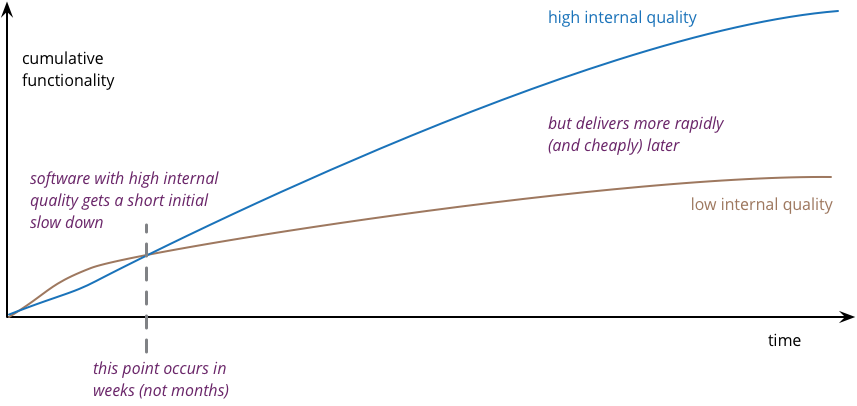
\includegraphics[width=1\textwidth]{./images/QASoftwareCompare.png}
        \caption{Vergleich einer guten und einer schlecten Softwarearchitektur}
        \label{fig:flow around cylinder}
        \source{https://martinfowler.com/articles/is-quality-worth-cost.html}
    \end{figure}

    Diese Eigenschaft muss man immer beim Projektbegin beachten, denn es wäre sehr Zeitaufwändig für ein Studiumprojekt, 
    für das man evtl. nur 1 Woche Zeit komplexe Architektur zu implementieren, die ohne jeglichen Funktionalitäten mehrere Wochen gebrauchen wird.

    Wenn man aber ein Projekt hat, das regelmäßig weiterentwickeln wird, dass man gleich eine gute Architektur umzusetzt.

    \subsection{Wichtigkeit der Testbarkeit der Software}
    Jedes Teil der Software wird in seinem Lebenszyklus mehrmals geändert. 
    Um die Funktionalität der neuen Version zu verifizieren, muss sie getestet werden.
    Man ist sehr daran interessiert diese Aufgabe zu automatisieren. 
    Wie in den früheren Kapitels bereits beschrieben wurde, am schnellsten findet man die Bugs, falls vorhanden, mit Unittests. 
    Bei den Unittests müssen die Module (z.B. einzelne Klassen in Falle von OOP Sprachen) in verschiedensten Umgebungen überprüft werden. 
    Das heißt, dass die Zustände von benutzten Modulen müssen leicht simulierbar sein.
    Dies erfordert eine Planung der Softwarearchitektur im Voraus, 
    um diese Eigenschaft zu implementieren um im Laufe der Entwicklung viel Zeit durch automatisierte Tests zu sparen.

    \subsection{Technische Umsetzung der Software Architektur}
    \subsubsection{Auswahl der Datenbank}
    \subsubsection{Dependency Rule}
    \subsubsection{Unterschied zu Layered Architektur}
    \subsubsection{Implementierung der Testbarkeit}
    - Humble Objects
    \subsubsection{Dependency Injection}
    In dem unteren Diagramm sieht man ein Beispiel von einer Anwendug, die die von der konsole ankommenden Zahlen quadriert und das Ergebnis zurückgibt.
    
    \begin{figure}[H]
        \centering
        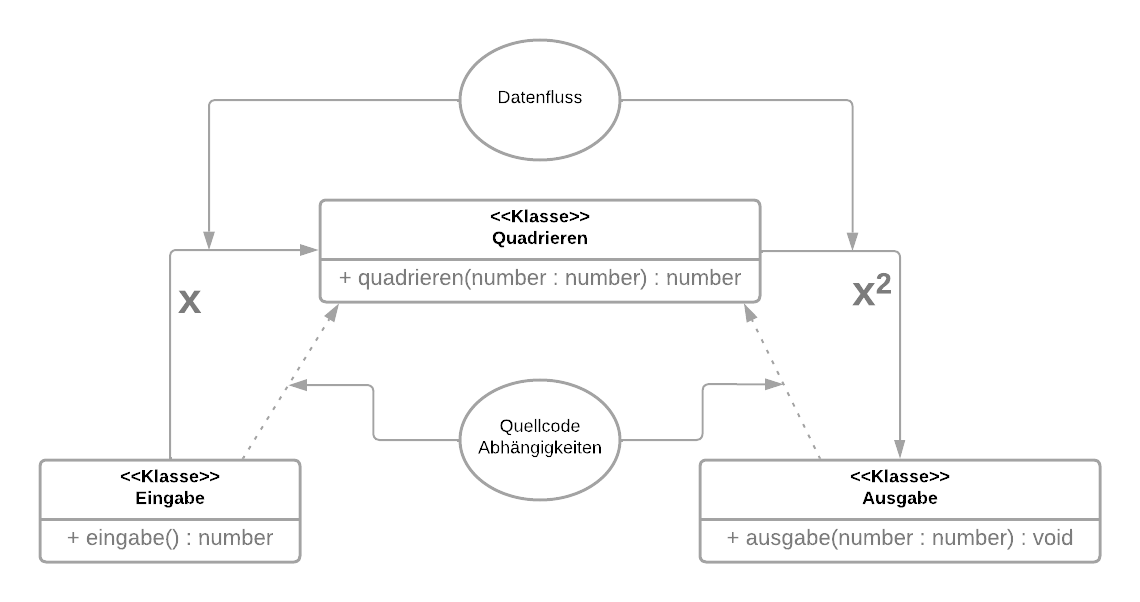
\includegraphics[width=1\textwidth]{./images/DepInj_1.png}
        \caption{Datenfluss und Quellcode Abhängigkeiten}
        \label{fig:flow around cylinder}
        \source{Eigene Quelle}
    \end{figure}

    Die Funktion "Quadrieren" ist in dem Fall befindet sich auf einem höheren Niveau als Eingabe und Ausgabe, 
    da das Quadrieren einer Zahl soll unabhängig von der Eingabe und Ausgabe sein.

    Würde man aber bei der Ausgabe die Eingabeparameter von ``number'' auf ``string'' ändern, so müsste man auch die Ausgabe von Quadrieren von ``number'' auf ``string'' ändern.
    Dies könnte auch eine weitere Kette an Anderungen im Programm auslösen. Zum Beispiel müssen auch die Unittests von ``Quadrieren'' geändert werden.
    Somit ist ``Quadrieren'' abhängig von der ``Ausgabe''

    Das Problem lässt sich mittels Dependency Injection lösen.
    In OOP Sprachen kann man dafür ``Interface'' benutzen.

    Die Lösung wurde dann so aussehen. 
    \begin{figure}[H]
        \centering
        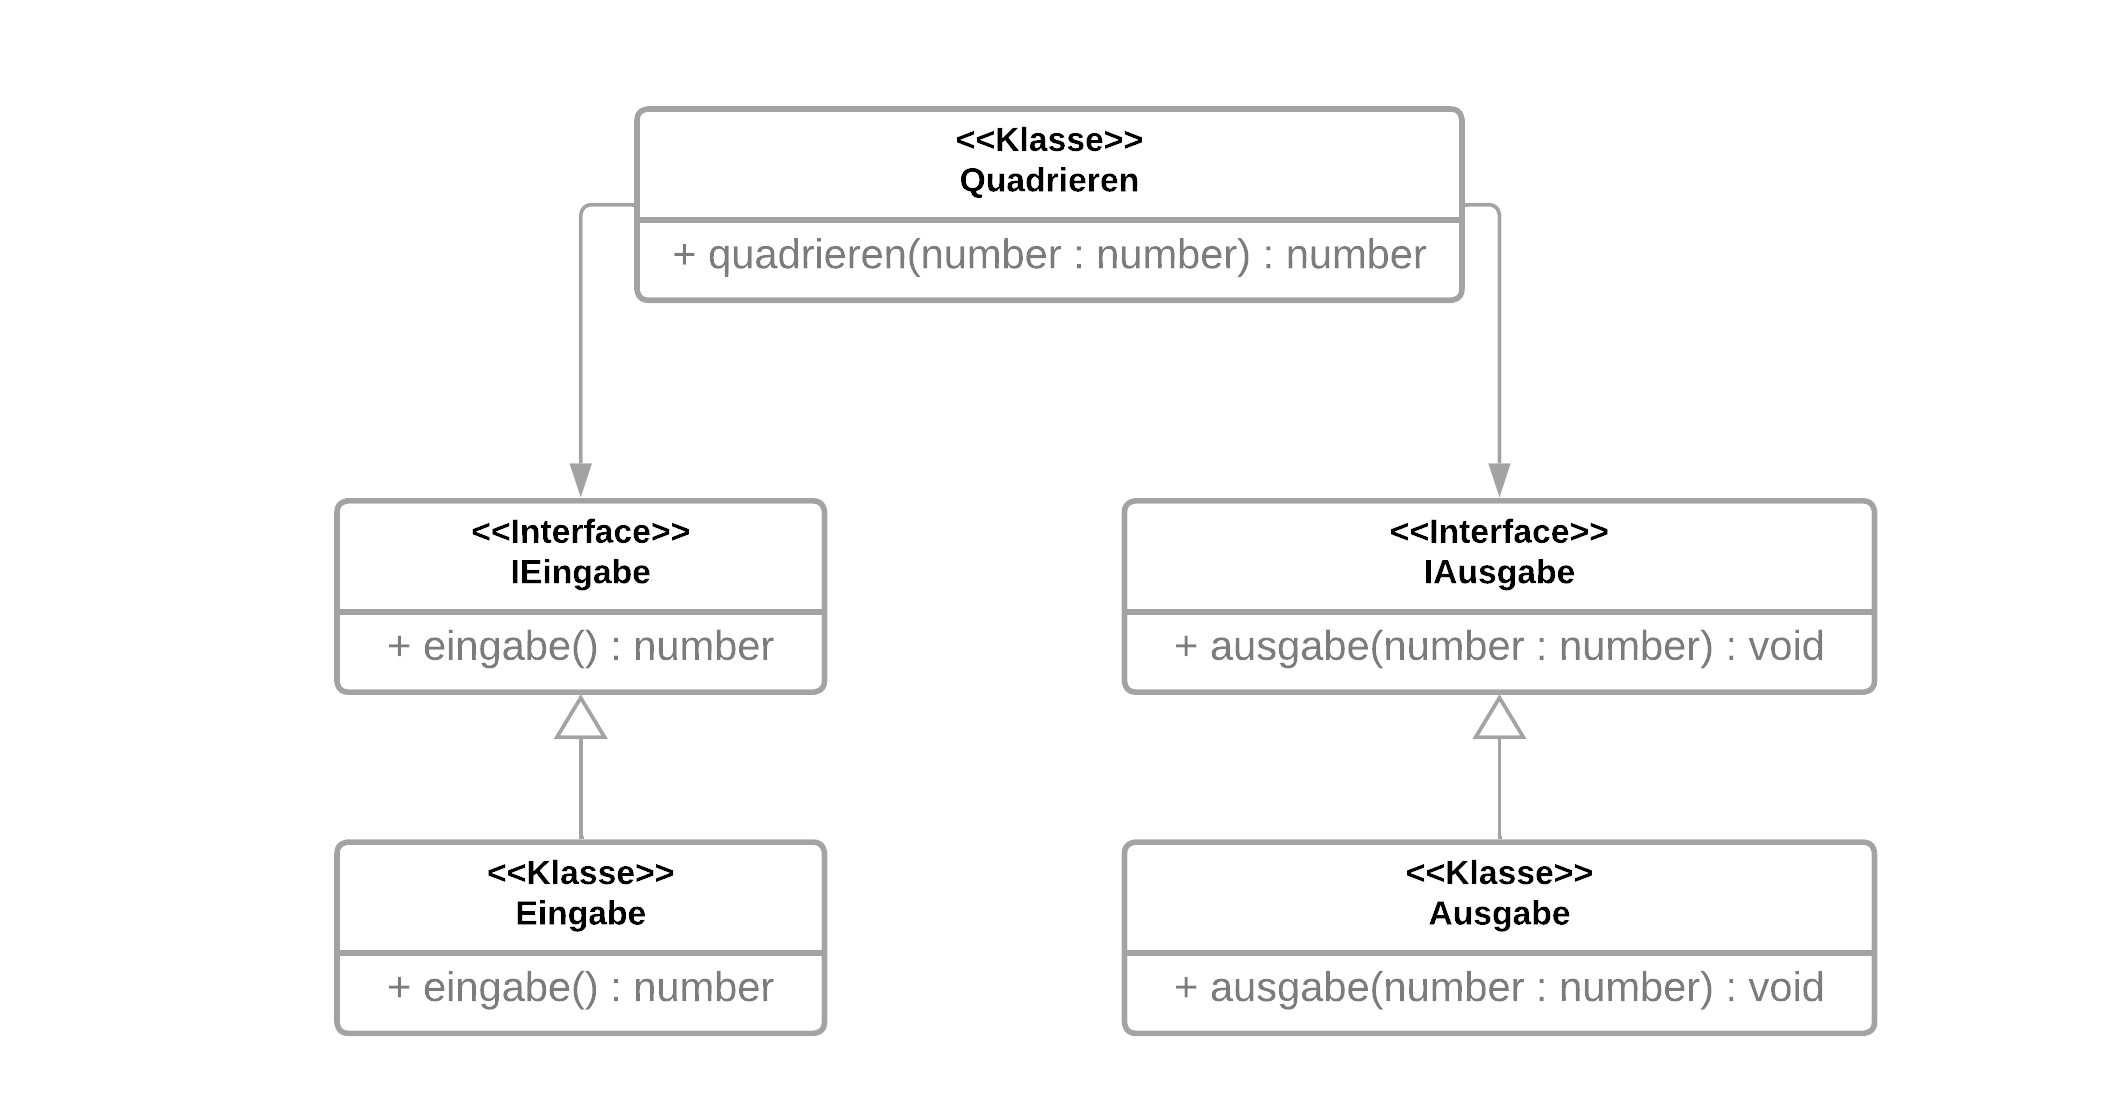
\includegraphics[width=1\textwidth]{./images/DepInj_2.png}
        \caption{Entkopplung der Abhängigkeiten}
        \label{fig:flow around cylinder}
        \source{Eigene Quelle}
    \end{figure}

    Dies lässt sich mit ``Interface'' (für OOP Sprachen) umsetzen, 
    in dem es frühestens bei der Initialisiereung der ``Quadrieren'' Klasse die jeweilige Eingabe und Ausgabe Klasse übergeben wird.

    Somit lässt sich die Funktion ``Quadrieren'' mit gefälschten Eingabe- und Ausgabeklasse mit Unit tests getestet werden.

    Wenn man alle Klassen über Interface miteinander verbindet, ist es möglich, dass die Umgebung von jeder einzelnen Klasse bei den Unittests gefälscht
    wird und somit das Schreiben von Unittests sehr einfach wird. 

    Interfaces können sich natürlich auch ändern und dann muss man auch alle davon betroffenen Objekte entsprechend ändern, 
    jedoch das passiert deutlich seltener als Änderung einer Klasse.

    Auch mit Dependency Injection lassen sich externe Schnittstellen wie Datenbank oder Netzwerkschnittstellen schnell austauschen, 
    denn man muss nur eine Klasse schreiben, die das Interface implementiert.


    


\newpage



% Example section added from an external tex-file, here located in ./Sections/
\import{./Sections/}{Aufgabestellung}

\import{./Sections/}{Loesung}


% Beschreibung der gewünschten Implementierung
\newpage
\import{./Sections/}{Bestinterface}

% Beschreibung der Implementierung der Software
\newpage
\import{./Sections/}{Implementierung}

% Example section added directly into the main-file
\section{Conclusion}
\textit{But the fact that some geniuses were laughed at does not imply that all who are laughed at are geniuses. They laughed at Columbus, they laughed at Fulton, they laughed at the Wright Brothers. But they also laughed at Bozo the Clown} -  \textcite{sagan_1993}.

% Printing bibliography
\newpage
\printbibliography[heading = bibintoc, title = Bibliography]    % 'bibintoc' inserts our bibliography into the table of contents

% Inserting appendix with separate settings
\addappendix
\import{./Appendices/}{example_appendix}

% End of document
\end{document}
